% Two national name ranges at issue. (a) Kombissiri, a four-digit name shared by six areas of the commune of
% Kombissiri: one frozen block each, laid end to end from 1000, each split into its main part and its tail
% reserve; the rest of the range is spare. (b) Koulouba, a four-digit name with one area: the numbers issued,
% the free numbers of the main part, the tail reserve and the spare. Data: kombissiri.dat, register.json.
\documentclass[tikz,border=2mm]{standalone}
\usepackage{fontspec}\setmainfont{LibertinusSans}[Extension=.otf,UprightFont=*-Regular,BoldFont=*-Bold,ItalicFont=*-Italic]
\usepackage{pgfplots}\pgfplotsset{compat=1.18}
\usepackage{pgfplotstable}
\definecolor{ink}{HTML}{A3121C}\definecolor{inkmid}{HTML}{D9584F}\definecolor{inklight}{HTML}{F2B8B3}\definecolor{inkpale}{HTML}{FBE3E1}
\definecolor{slate}{HTML}{8C9AA6}\definecolor{grid}{HTML}{DADDE0}
\providecommand{\T}[2]{\ifdefined\paperfr #2\else #1\fi}
\usetikzlibrary{patterns}
\begin{document}
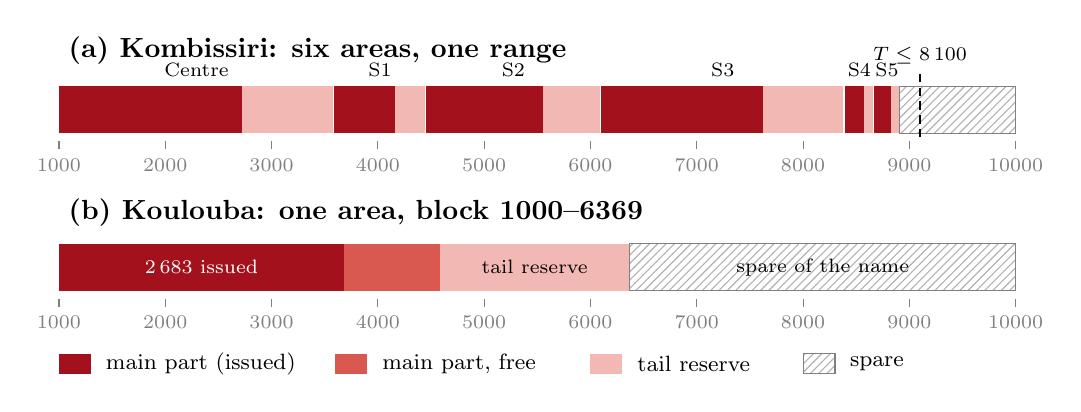
\begin{tikzpicture}[font=\footnotesize, x=1.35mm, y=1cm]
% one unit of x = 100 numbers; the range 1000-9999 spans 90 units
\newcommand{\nx}[1]{(#1-1000)/100}
\foreach \v in {1000,2000,...,9000,10000} {
  \draw[gray] ({\nx{\v}},-0.1) -- ({\nx{\v}},-0.2) node[below, font=\scriptsize] {\pgfmathparse{int(\v)}\pgfmathresult};
  \draw[gray] ({\nx{\v}},-2.1) -- ({\nx{\v}},-2.2) node[below, font=\scriptsize] {\pgfmathparse{int(\v)}\pgfmathresult};}
\node[anchor=west, font=\bfseries] at (0,1.05) {(a) Kombissiri: \T{six areas, one range}{six aires, une plage}};
\foreach \lo/\hi/\lab in {1000/3589/{Centre}, 3590/4449/S1, 4450/6099/S2, 6100/8389/S3, 8390/8669/S4, 8670/8909/S5} {
  \pgfmathsetmacro{\m}{\lo+floor(2*(\hi-\lo+1)/3)}
  \fill[ink] ({\nx{\lo}},0) rectangle ({\nx{\m}},0.6);
  \fill[inklight] ({\nx{\m}},0) rectangle ({\nx{\hi+1}},0.6);
  \draw[white, line width=0.8pt] ({\nx{\hi+1}},0) -- ({\nx{\hi+1}},0.6);
  \node[above, font=\scriptsize] at ({(\nx{\lo}+\nx{\hi+1})/2},0.6) {\lab};}
\draw[gray, pattern=north east lines, pattern color=gray!60] ({\nx{8910}},0) rectangle ({\nx{10000}},0.6);
\draw[densely dashed] ({\nx{9100}},-0.05) -- ({\nx{9100}},0.75) node[above, font=\scriptsize, align=center] {$T \le 8\,100$};
\node[anchor=west, font=\bfseries] at (0,-1.0) {(b) Koulouba: \T{one area, block 1000--6369}{une aire, bloc 1000--6369}};
\fill[ink] (0,-2) rectangle ({\nx{3683}},-1.4);
\fill[inkmid] ({\nx{3683}},-2) rectangle ({\nx{4580}},-1.4);
\fill[inklight] ({\nx{4580}},-2) rectangle ({\nx{6370}},-1.4);
\draw[gray, pattern=north east lines, pattern color=gray!60] ({\nx{6370}},-2) rectangle ({\nx{10000}},-1.4);
\node[font=\scriptsize, white] at ({\nx{2341}},-1.7) {\T{2\,683 issued}{2\,683 émis}};
\node[font=\scriptsize, align=center] at ({\nx{5475}},-1.7) {\T{tail reserve}{réserve de fin}};
\node[font=\scriptsize] at ({\nx{8185}},-1.7) {\T{spare of the name}{réserve du nom}};
% legend
\begin{scope}[shift={(0,-3.05)}]
  \fill[ink] (0,0) rectangle (3,0.25); \node[anchor=west] at (3.5,0.125) {\T{main part (issued)}{partie principale (émis)}};
  \fill[inkmid] (26,0) rectangle (29,0.25); \node[anchor=west] at (29.5,0.125) {\T{main part, free}{partie principale, libre}};
  \fill[inklight] (50,0) rectangle (53,0.25); \node[anchor=west] at (53.5,0.125) {\T{tail reserve}{réserve de fin}};
  \draw[gray, pattern=north east lines, pattern color=gray!60] (70,0) rectangle (73,0.25); \node[anchor=west] at (73.5,0.125) {\T{spare}{réserve}};
\end{scope}
\end{tikzpicture}
\end{document}
